\documentclass[14pt]{article}
\usepackage{makeidx}
\usepackage{multirow}
\usepackage{multicol}
\usepackage[dvipsnames,svgnames,table]{xcolor}
\usepackage{graphicx}
\usepackage{epstopdf}
\usepackage{ulem}
\usepackage{hyperref}
\usepackage{amsmath}
\usepackage{amssymb}
\author{Omkar Mohite}
\title{}
\usepackage[paperwidth=595pt,paperheight=841pt,top=72pt,right=72pt,bottom=72pt,left=72pt]{geometry}

\makeatletter
	\newenvironment{indentation}[3]%
	{\par\setlength{\parindent}{#3}
	\setlength{\leftmargin}{#1}       \setlength{\rightmargin}{#2}%
	\advance\linewidth -\leftmargin       \advance\linewidth -\rightmargin%
	\advance\@totalleftmargin\leftmargin  \@setpar{{\@@par}}%
	\parshape 1\@totalleftmargin \linewidth\ignorespaces}{\par}%
\makeatother 

% new LaTeX commands


\begin{document}


\begin{center}
{\Large Project Title:}
\end{center}

\begin{center}
{\Huge \textbf{Controlling Firebird V using EEG sensor (Brainwave sensor)}\\}
\end{center}

\begin{center}

\end{center}
\begin{center}
{\LARGE Interns:}

\begin{enumerate}
	\item {\LARGE \textbf{Omkar Rajendra Mohite}}


{\raggedright
{\Large Email id:
\href{mailto:mohiteomkar46@gmail.com}{mohiteomkar46@gmail.com}}
}

{\raggedright
{\Large Contact No.: +91 9820774749}
}


	\item {\LARGE \textbf{Ashish Kumar Jain}}


{\raggedright
{\Large Email id:
\href{mailto:ashishkumarjain8888@gmail.com}{ashishkumarjain8888@gmail.com}}
}


{\raggedright
{\Large Contact No.: +91 8800470934}
}
\end{enumerate}
\begin{center}
{\LARGE Mentors:}
\end{center}

\begin{enumerate}
	\item {\LARGE     \textbf{Mehul Makwana}}


{\raggedright
{\Large     Email id:
\href{mailto:mehul.makwan@gmail.com}{mehul.makwan@gmail.com}}
}

{\raggedright
{\Large     Contact No.: +91 9405624900}
}


	\item {\LARGE     \textbf{Rutuja Ekatpure}}


{\raggedright
{\LARGE     }{\Large Email id:}
}

{\raggedright
{\Large     Contact No.:}
}
\end{enumerate}
\end{center}
\begin{center}
{\large Duration of Internship:}
\end{center}

\begin{center}
\textbf{{\LARGE 25$^{th}$ May 2015 to 8$^{th}$ July 2015}}
\end{center}
\break
\begin{center}
{\Huge Abstract}
\end{center}

{\large If suppose using our attention and meditation power we could control any specific activity then it would reduce the human effort. With increase in field of technology everything is obtained very easily. This has made a normal person go away from understanding what his/her brain can achieve. This project of ‘Controlling Firebird V using EEG sensor’ is a prototype of controlling any activity using concentration power of human. In this project, Neurosky Mindwave mobile is used as EEG sensor which measures attention and meditation power of a person. This data is manipulated and made to control Firebird V. Bluetooth is used as a medium to communicate from sensor to bot. The velocity of forward motion is varied depending upon the attention level of the person, while detection of two eye-blinks will make the bot rotate left. The left motion continues until the third eye-blink is detected making the bot move forward again depending upon the velocity which is proportional to the attention level of the user. When the sensor is removed from head, the bot stops to move.}

\break
\begin{center}
{\Huge Introduction}
\end{center}
We are living in 21$^{st}$ century-an era for automation, modern technology. In India nearly 1.5\% of total population are affected by paralysis. In America 1.9\% of total population is affected by paralysis. In paralysis the crucial condition is not able to move any of the body part. 
Around 1 out of 50 children is mentally challenged all over the world according to data calculated in 2013. Considering these conditions, this project is developed in order to help reduce the effort for paralysed people and to increase the mind capacity of the mentally challenged children.
\begin{center}
	\graphicspath{ {images/} }
	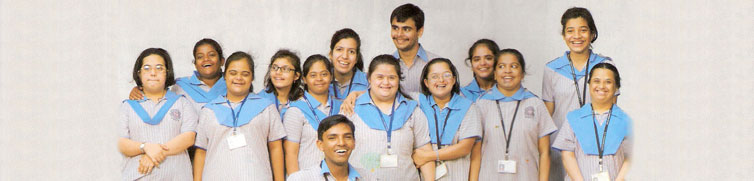
\includegraphics[width=16cm, height=4cm]{Mentally_challenged}
\end{center}
\begin{enumerate}
	\item \textbf{{\large About EEG:\\}}
Electroencephalography (EEG) is a non-invasive method to record electrical activity of the brain along the scalp. EEG measures voltage fluctuations resulting from ionic current within the neurons of the brain. In clinical contexts, EEG refers to the recording of the brain's spontaneous electrical activity over a period of time, as recorded from multiple electrodes placed on the scalp.


The brain's electrical charge is maintained by billions of neurons. Neurons are electrically charged (or "polarized") by membrane transport proteins that pump ions across their membranes. Neurons are constantly exchanging ions with the extracellular milieu, for example to maintain resting potential and to propagate action potentials. Ions of similar charge repel each other, and when many ions are pushed out of many neurons at the same time, they can push their neighbours, who push their neighbours, and so on, in a wave. This process is known as volume conduction. When the wave of ions reaches the electrodes on the scalp, they can push or pull electrons on the metal on the electrodes. Since metal conducts the push and pull of electrons easily, the difference in push or pull voltages between any two electrodes can be measured by a voltmeter. Recording these voltages over time gives us the EEG.


	\item \textbf{{\large About Brainwaves:}}
\begin{center}
	\graphicspath{ {images/} }
	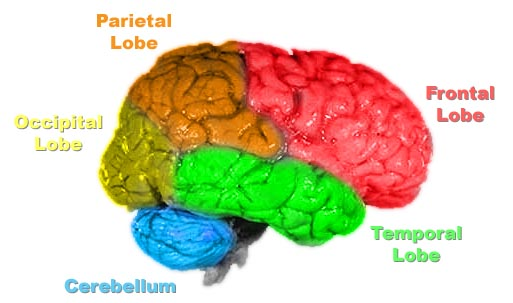
\includegraphics[width=15cm, height=8cm]{Brain-anatomy}
\end{center}

\begin{enumerate}
	\item \href{http://en.wikipedia.org/wiki/Gamma\_wave}{Gamma waves}~are oscillating waves with frequencies around 40 Hz, although they can be as high as 100 Hz and as low as 24 Hz. These originate from the thalamus (buried deep in the centre of the brain) and are responsible for states of high attention and concentration.
	\item \href{http://en.wikipedia.org/wiki/Beta\_wave}{Beta waves}~are between 12 and 30 Hz and are the states associated with normal waking consciousness. These are emitted from the motor cortex, a region of the cerebral cortex, which is the outermost layer of tissue on the brain. Beta waves are split into three sections: Low Beta Waves (12.5-16 Hz, “Beta 1 power”); Beta Waves (16.5–20 Hz, “Beta 2 power”); and High Beta Waves (20.5-28 Hz, “Beta 3 power”).
	\item \href{http://en.wikipedia.org/wiki/Alpha\_wave}{Alpha waves}~originate at the Occipital lobe and have a frequency of 8-12Hz. These are most present when you are awake but are very drowsy or relaxed.
	\item \href{http://en.wikipedia.org/wiki/Theta\_wave}{Theta waves}~are oscillating waves that are located in the Hippocampus and are associated with dreaming. They are in the 4-7Hz range.
	\item \href{http://en.wikipedia.org/wiki/Delta\_wave}{Delta wavis}~are associated with very deep, dreamless sleep cycles and are high amplitude waves, which have a 0 to 3Hz frequency. These waves emit from both the thalamus and the cortex.
\end{enumerate}


	\item \textbf{{\large Objectives:}}
	\begin{enumerate}
	\item The main objective is to Control Firebird V bot using EEG sensor (brainwave sensor) which records the attention, meditation power and eye-blink of the user and not his/her thoughts.
	\item This theme can be implemented to control Wheelchair for paralyzed people.
	\item We can also play games in which the person with more concentration power wins.\\
\end{enumerate}


	\item \textbf{{\large Tasks performed and Deadlines:}}
\end{enumerate}

{\raggedright

\vspace{3pt} \noindent
\begin{tabular}{|p{40pt}|p{311pt}|p{70pt}|}
\hline
\parbox{40pt}{\centering 
\textbf{Sr. No.}
} & \parbox{311pt}{\centering 
\textbf{Tasks}
} & \parbox{70pt}{\centering 
\textbf{Deadlines}
} \\
\hline
\parbox{40pt}{\centering 
1.
} & \parbox{311pt}{\raggedright 
Understanding Brainwaves and about EEG sensor(Mindwave mobile headset)
} & \parbox{70pt}{\centering 
3 days
} \\
\hline
\parbox{40pt}{\centering 
2.
} & \parbox{311pt}{\raggedright 
Configuring bluetooth module with sensor
} & \parbox{70pt}{\centering 
2 days
} \\
\hline
\parbox{40pt}{\centering 
3.
} & \parbox{311pt}{\raggedright 
Avalysing and Processing Brainwave values.
} & \parbox{70pt}{\centering 
4 days
} \\
\hline
\parbox{40pt}{\centering 
4.
} & \parbox{311pt}{\raggedright 
Interfacing Sensor to Firebird V via BVuetooth.
} & \parbox{70pt}{\centering 
3 days
} \\
\hline
\parbox{40pt}{\centering 
5.
} & \parbox{311pt}{\raggedright 
LED Bar graph blinking based on Attention level
} & \parbox{70pt}{\centering 
5 days
} \\
\hline
\parbox{40pt}{\centering 
6.
} & \parbox{311pt}{\raggedright 
Controlling Firebird V motions using attention level and eye-blink
} & \parbox{70pt}{\centering 
6 days
} \\
\hline
\parbox{40pt}{\centering 
7.
} & \parbox{311pt}{\raggedright 
Documentation
} & \parbox{70pt}{\centering 
5 days
} \\
\hline
\end{tabular}
\vspace{2pt}

}

\break

\begin{center}
{\Huge Block Diagram}
\end{center}
\begin{center}
	\graphicspath{ {images/} }
	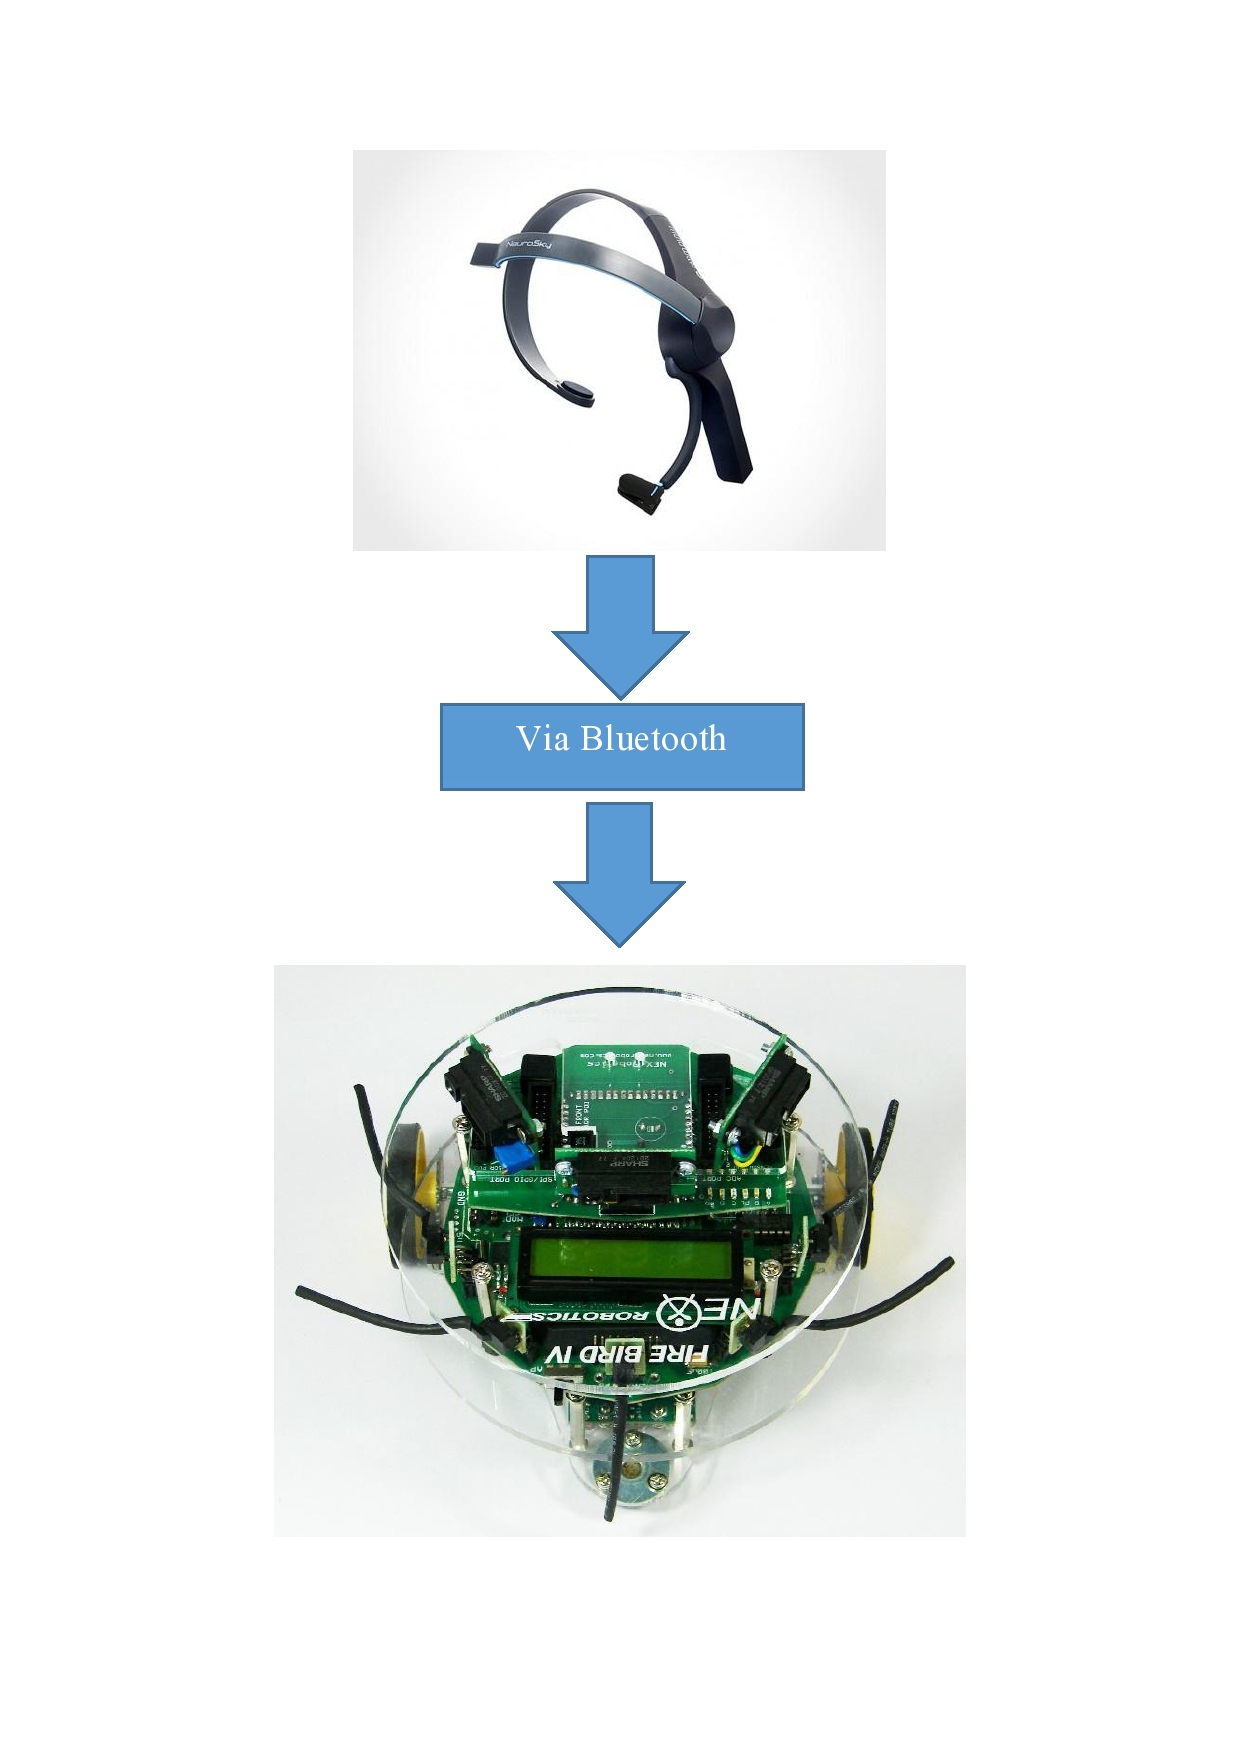
\includegraphics[width=17cm, height=21cm]{Block_diagram}
\end{center}
\begin{itemize}
	\item Velocity proportional to Attention level of the person.
	\item Two eye-blink will give left turn continuously.
	\item Furthermore one eye-blink will again make bot to move forward.
\end{itemize}

\break

\begin{center}
{\Huge Working of the project}
\end{center}

Neurosky Mindwave headset (Brainwave sensor) communicates with the help of data packets. Following is the pattern in which data bytes are sent:

{\raggedright
[SYNC] [SYNC] [PLENGTH]      [PAYLOAD...]     [CHKSUM]
}

{\raggedright
\_\_\_\_\_\_\_\_\_\_\_\_\_\_\_\_\_\_\_\_\_\_\_\_\_\_\_\_\_\_\_\_\_\_\_\_\_     \_\_\_\_\_\_\_\_\_\_\_\_\_\_\_\_\_\_\_
    \_\_\_\_\_\_\_\_\_\_\_\_
}

{\raggedright
\textasciicircum{}\textasciicircum{}\textasciicircum{}\textasciicircum{}\textasciicircum{}\textasciicircum{}\textasciicircum{}\textasciicircum{}
(Header)
\textasciicircum{}\textasciicircum{}\textasciicircum{}\textasciicircum{}\textasciicircum{}\textasciicircum{}\textasciicircum{}
       \textasciicircum{}\textasciicircum{} (Payload)
\textasciicircum{}\textasciicircum{}     \textasciicircum{} (Checksum)
\textasciicircum{}
}

The two [SYNC] bytes are used to signal the beginning of a new arriving Packet and are bytes with the value 0xAA (decimal 170). Synchronization is two bytes long, instead of only one, to reduce the chance that [SYNC] (0xAA) bytes occurring within the Packet could be mistaken for the beginning of a Packet.
The [PLENGTH] byte indicates the length, in bytes, of the Packet's Data Payload [PAYLOAD] section, and may be any value from 0 up to 169. Any higher value indicates an error (PLENGTH TOO LARGE). Be sure to note that [PLENGTH] is the length of the Packet's Data Payload, NOT of the entire Packet. The Packet's complete length will always be [PLENGTH] + 4.


The [CHKSUM] Byte must be used to verify the integrity of the Packet's Data Payload. The Payload's Checksum is defined as:

\begin{itemize}
	\item summing all the bytes of the Packet's Data Payload
	\item taking the lowest 8 bits of the sum
	\item performing the bit inverse (one's compliment inverse) on those lowest 8 bits
\end{itemize}

{\raggedright
Program the bot according to the data packets being received.
}

{\raggedright
Following are the analysed data from the Neurosky Mindwave mobile:
}

\begin{itemize}
	\item We obtain only two types of data packets. Payload length of 0x04 and 0x20. 
	\item The 0x04 payload length data packet consists of raw values which indicates mainly the connection of headset on head, pairing values, and eye-blink data values which are send when scalp touched to cathode and anode are moved.
	\item The 0x20 payload length data packet consists of poor quality indication, attention level indication and meditation level indication.
	\item 0x02 indicates poor quality detection. The next byte to that indicates poor quality signal level. For eye-blink detection this value should be 0.
	\item 0x04 indicates attention level detection. The next byte to that indicates level of attention.
	\item 0x05 indicates meditation level detection. The byte next to 0x05 indicates meditation level achieved.
	\item 0x02 always appear next to 0x20 i.e. next to payload length.
	\item 0x04 always appear at 28$^{th}$ position of payload data and 0x05 always appear
at 30$^{th}$ position of payload data.
	\item For attention, meditation and poor quality detection 0x20 byte long payload data is useful.
	\item For eye-blink detection 0x04 byte long payload data is useful.
\end{itemize}

Thus by using above analysed data Firebird V is programmed to move forward according to attention level and turn left depending upon eye-blink strength.

\break

\begin{center}
{\Huge Progarm Description}
\end{center}

\textbf{{\large Program to display Attention level of a person on LED bargraph and give the velocity of bot depending on it. Rotate left after detection to two eye-blinks..}}

\begin{enumerate}
	\item \textbf{{\large Algorithm:}}


\begin{enumerate}
	\item Initialize all required ports.
	\item Check for two consecutive SYNC bytes ‘AA’.
	\item Check for third byte which is the payload length.
	\item If payload length is 0x20, then store the next 32 bytes in an array. If payload length is 0x04 then move to step no. 11
	\item Calculate the generated checksum.
	\item If the last byte i.e. checksum byte of the data packet is equal to the generated checksum then check for 28th byte of the array.
	\item If 28th byte is 0x04, then attention detected.
	\item Then 29th byte indicates attention level of the person between 0-100.
	\item Give velocity to the bot depending on the attention level.
	\item Check for 1st byte of the array. If it is 0x02, then next byte to it should be 0x00, then eye-blink can be detected.
	\item If payload length is 0x04, then store the next 4 bytes in an array.
	\item Store the 1st and 2nd byte after 0x02 of the array in a variable and keep adding it for next 100 data packets.
	\item After taking average by 100, Eye-blink strength is between 110 and 350 and raw data values ranges above 350.
	\item Now repeat from step 11 and 12 three times and check the eye-blink strength.
	\item If eye- blink is given then its value will range between 110 and 350. 
	\item Detection of such two eye-blinks will turn the bot left.
	\item In order to stop the bot, remove the sensor from head. It will give values above 350.
	
\end{enumerate}

\break

	\item \textbf{{\large Flowchart:}}
\end{enumerate}
\begin{center}
	\graphicspath{ {images/} }
	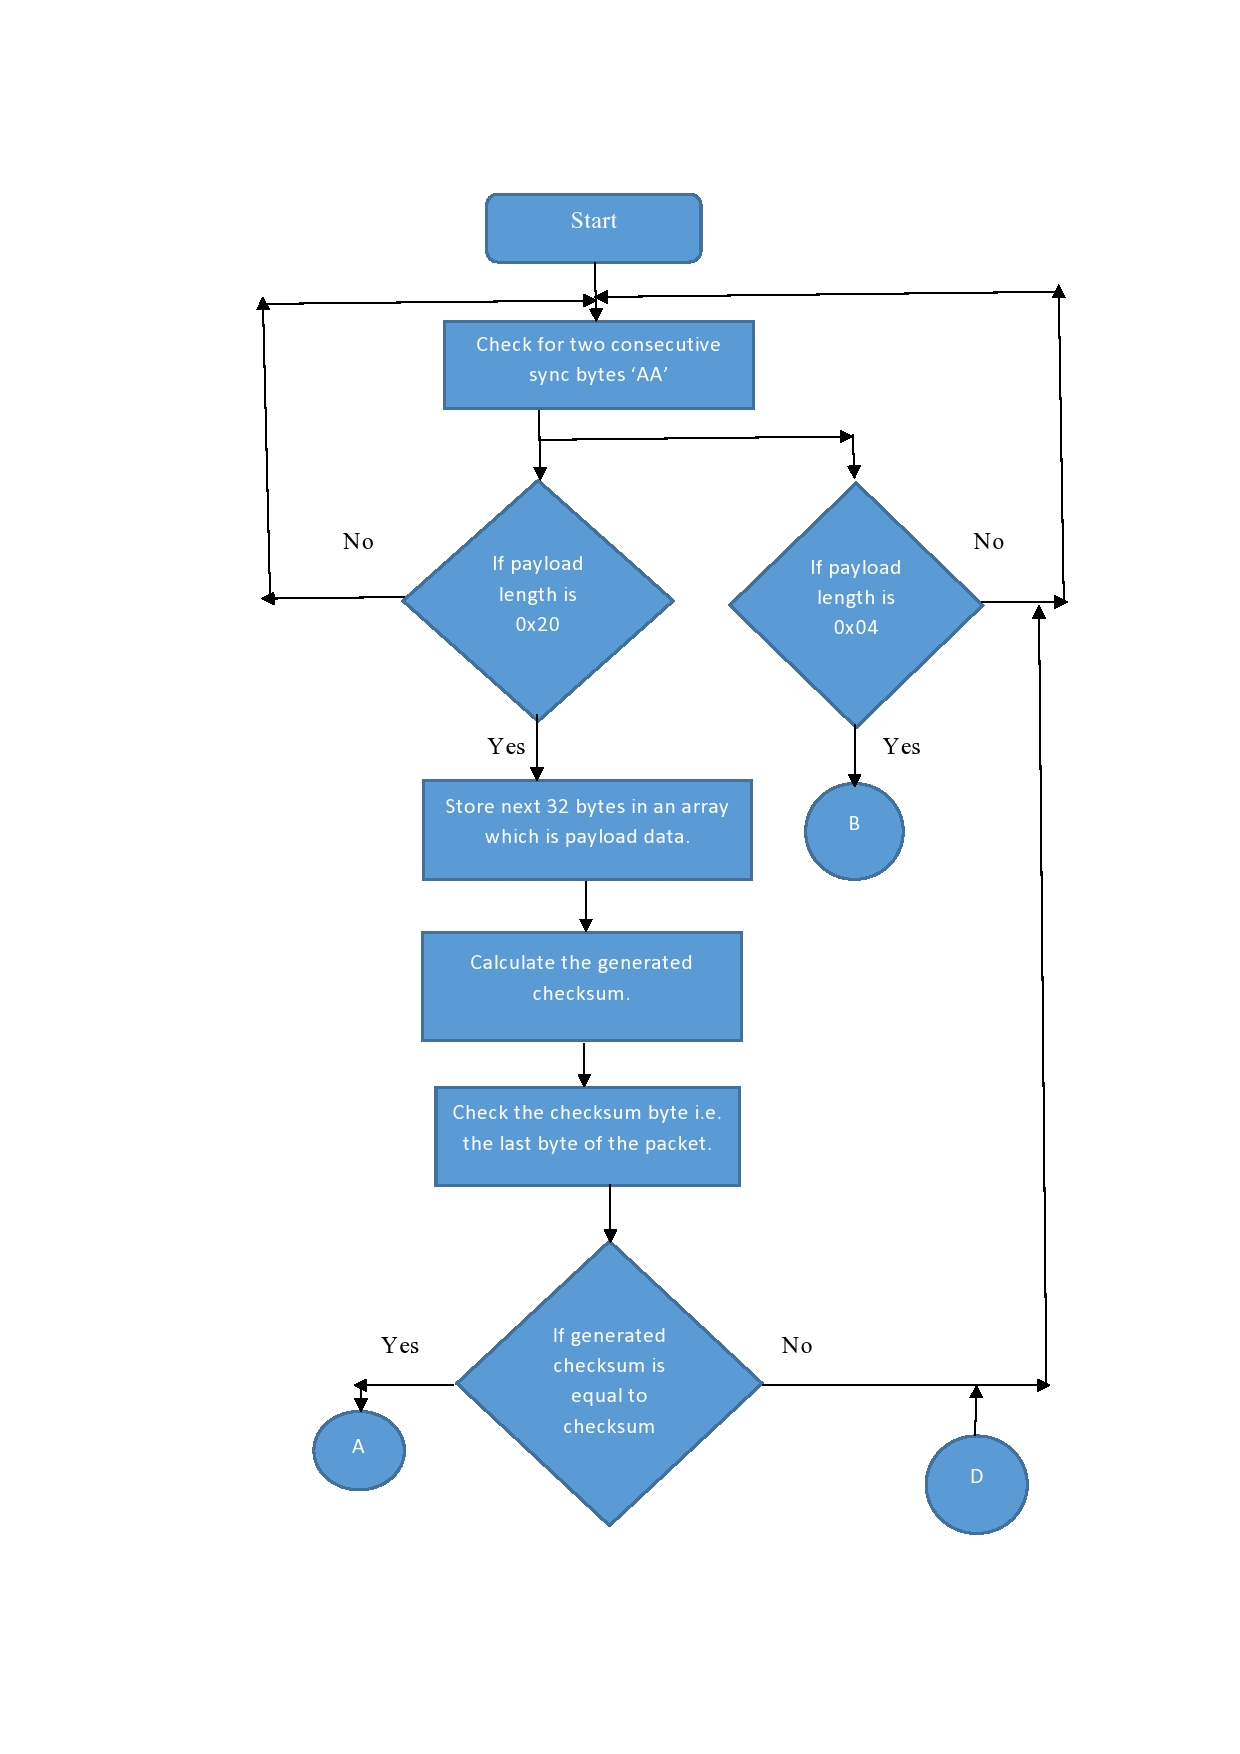
\includegraphics[width=18cm, height=23cm]{Flowchart1}
\end{center}
\begin{center}
	\graphicspath{ {images/} }
	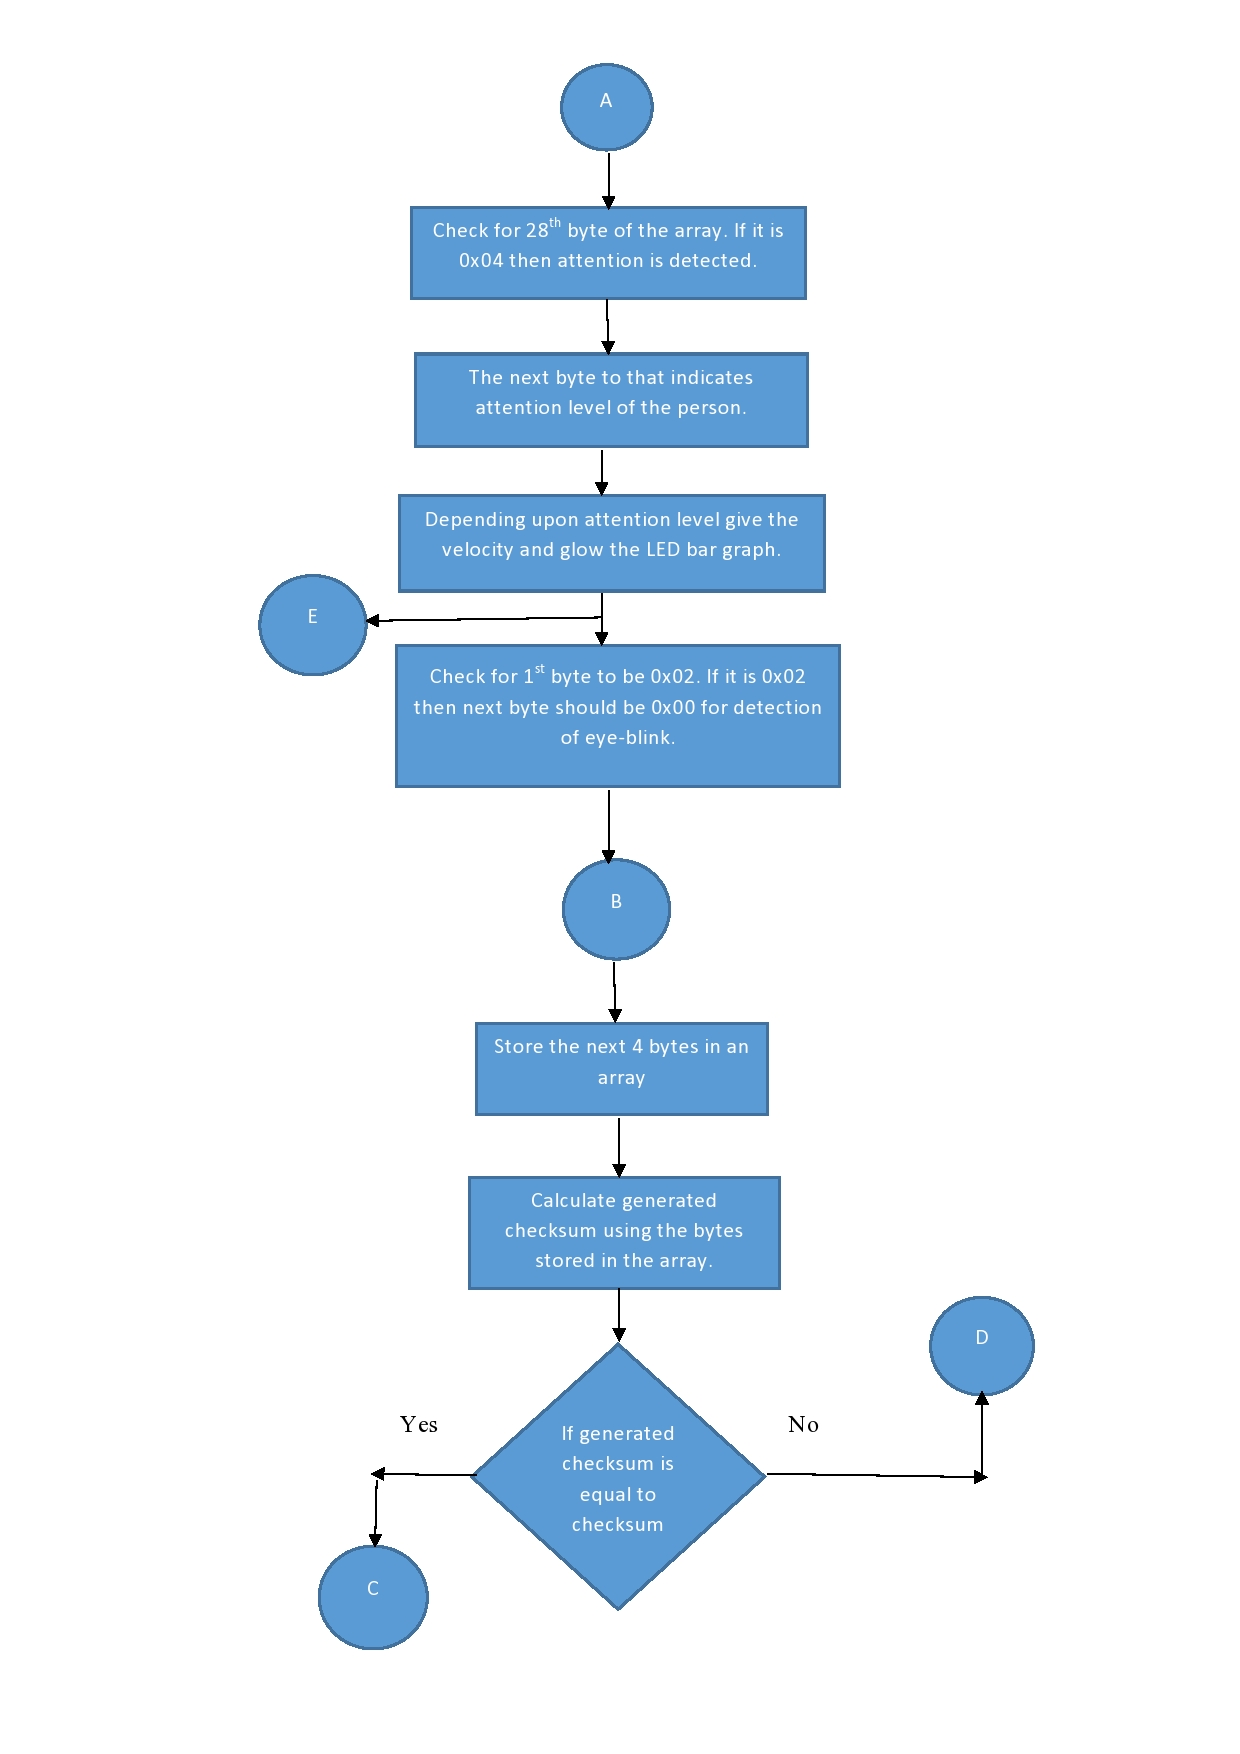
\includegraphics[width=18cm, height=24cm]{Flowchart2}
\end{center}
\begin{center}
	\graphicspath{ {images/} }
	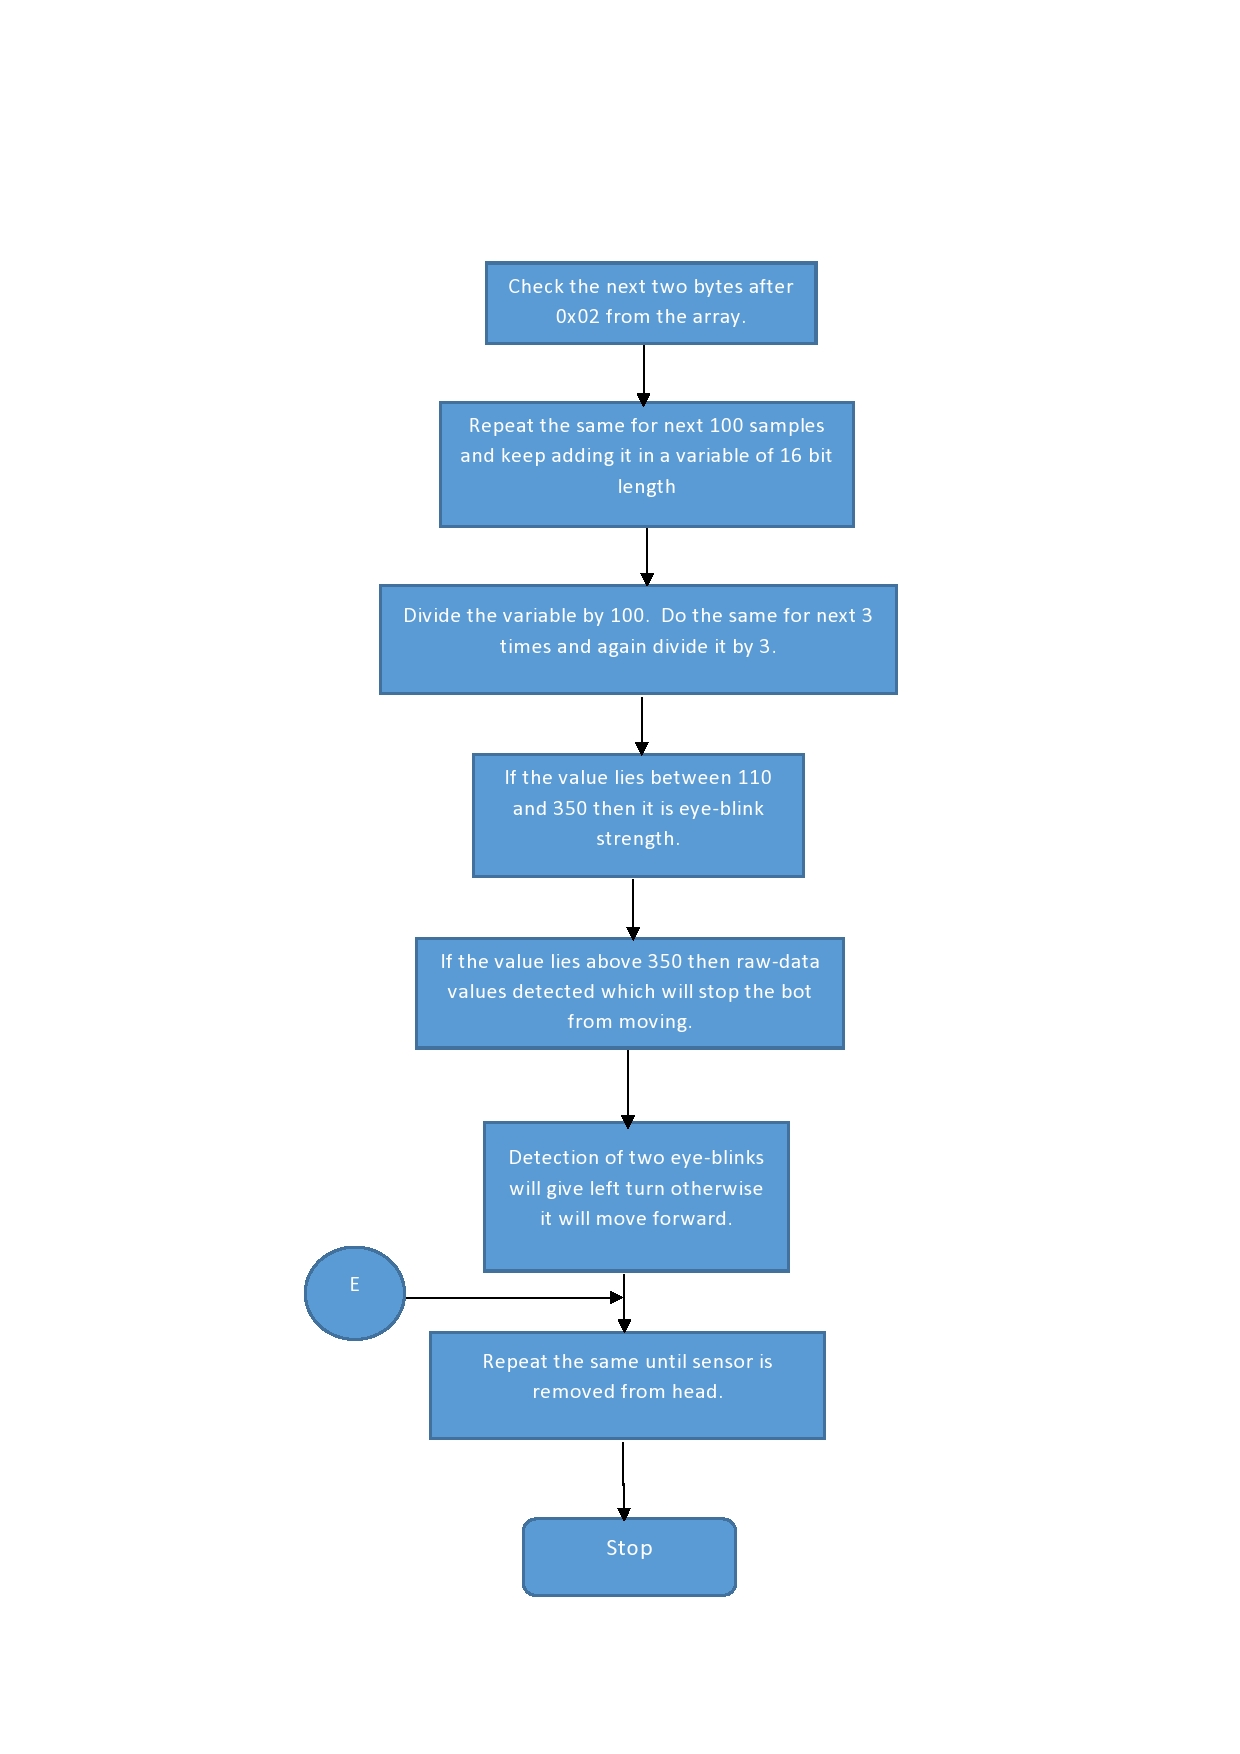
\includegraphics[width=18cm, height=24cm]{Flowchart3}
\end{center}

\break

\begin{center}
{\Huge Components and its Configuration}
\end{center}

\begin{enumerate}
	\item \textbf{{\large Bluetooth module (JY-MCU):}}


{\raggedright
This bluetooth module is interfaced on Firebird V robot. Following are the AT commands given:
}

\begin{itemize}
	\item AT
	\item AT+NAME=EEG
	\item AT+PSWD=0000
	\item AT+CMODE=0
	\item AT+UART=9600,0,0
	\item AT+ROLE=1
	\item AT+BIND=XXXX,YY,ZZZZZZ (Mindwave Unique Number (20:68:9d:88:c1:d7))
	\item AT+IAC=9E8B33
	\item AT+CLASS=0
	\item AT+INQM=1
\end{itemize}


	\item \textbf{{\large Firebird V connecniots:}}
	\begin{enumerate}
	\item Connect Bluetooth on Firebird V.
	\item Make use of expansion slot of UART connections.
	\item Connect to 37 and 38 pin no. of expansion slot. 37 pin no. indicates TXD and 38 pin no. indicates RXD.
	\item Connect RXD of bluetooth module to TXD of Firebird V and vice versa.
	\item Connect VCC to pin no.1 of and GND to pin no.2 of expansion slot.
	\item Now pair your headset with bluetooth module.
\end{enumerate}


	\item \textbf{{\large Neurosky Mindwave mobile:}}


This is an EEG sensor which communicates via bluetooth sending data packets.
\end{enumerate}

\break

\begin{center}
{\Huge Problems faced and resolved:}
\end{center}

\begin{enumerate}
	\item \textbf{UART problem:}

Initially we used UART 2 for interfacing bluetooth but it created the problem and half of data values were not getting received. This was because the same UART was used for bootloader.

\textbf{Solution:}

We changed the connection to UART 1 in the expansion slot.

\item \textbf{ISR problem:}


The given ISR SIGNAL(SIG\_USART1\_RECV) used to receive the incoming data and store in a variable. Mindwave mobile sends data at 512 symbols per second. Due to low processing speed most of the data values used to get lost.

\textbf{Solution:}
Instead of using a single variable to store the incoming data, we used buffer were data values were stored without getting lost.

	\item \textbf{Eye-bink data values:}


The eye-blink data values are similar to the raw-data values when sensor is removed from the head. So to distinguish between them is the problem faced.
\end{enumerate}

\break

\begin{center}
{\Huge Future Scope}
\end{center}

\begin{itemize}
	\item In the society there are many children around who are mentally disabled and cannot have their mind stable. If there is a game available for them in which they are made to control a robot or a car according to the attention and meditation power then they will try to control it. This might increase their concentration power over a period of time if they practice it every day.
\end{itemize}

\begin{itemize}
	\item Similarly Paralysed people who cannot move their body parts can be able to control their wheelchair using their attention level and eye-blink.
\end{itemize}

\begin{itemize}
	\item Using this project if we make game based on the attention and meditation level of a person, there will be definitely growth in his/her mental ability.
\end{itemize}

\break

\begin{center}
{\Huge References}
\end{center}

\begin{itemize}
	\item Firebird V hardware and software manuals.
	\item Neurosky Mindwave Headset datasheets.
	\item JY-MCU and HC-05 Bluetooth module datasheets.
	\item \href{https://en.wikipedia.org/wiki/Electroencephalography}{https://en.wikipedia.org/wiki/Electroencephalography}
	\item \href{http://neurosky.com/biosensors/eeg-sensor/biosensors/}{http://neurosky.com/biosensors/eeg-sensor/biosensors/}
	\item \href{https://learn.sparkfun.com/tutorials/hackers-in-residence---hacking-mindwave-mobile}{https://learn.sparkfun.com/tutorials/hackers-in-residence---hacking-mindwave-mobile}
	\item \href{https://www.pantechsolutions.net/mind-attention-control-led-using-arduino}{https://www.pantechsolutions.net/mind-attention-control-led-using-arduino}
	\item \href{https://www.pantechsolutions.net/mind-meditation-control-led-using-arduino}{https://www.pantechsolutions.net/mind-meditation-control-led-using-arduino}
	\item \href{https://www.pantechsolutions.net/eye-blink-control-led-using-arduino}{https://www.pantechsolutions.net/eye-blink-control-led-using-arduino}
\end{itemize}
\hspace{15pt}

\begin{center}
	{\Huge Softwares used:}
\end{center}
\begin{itemize}
	\item Atmel Studio 6.0
	\item AVR bootloader
	\item Arduino
	\item Arduino Processing
\end{itemize}

\end{document}